\documentclass{beamer}

% Theme selection
\usetheme{Madrid}
\usecolortheme{default}

% Packages
\usepackage{graphicx}
\usepackage{booktabs}
\usepackage{amsmath}
\usepackage{amssymb}
\usepackage{braket} % For Dirac notation
\usepackage{lmodern} % Fixes font size warnings
\usepackage{algorithm}
\usepackage{algpseudocode}
\graphicspath{{../}} % Images are in the parent directory

% Title Information
\title[Optimasi Portofolio via HE-VQE]{Integrasi Econophysics, Game Theory, dan Variational Quantum Eigensolver (VQE) untuk Optimasi Portofolio}
\subtitle{Studi Kasus Pemilihan 2 Aset Terbaik dari 4 Aset}
\date{\today}

\begin{document}

% Slide 1: Title Page
\frame{\titlepage}



% Slide 2: Metodologi / Pipeline Lengkap
\begin{frame}{Metodologi: Pipeline Lengkap}
    Visualisasi alur kerja:
    \begin{enumerate}
        \item \textbf{Data Acquisition}: Pengambilan data historis saham LQ45 (yfinance).
        \item \textbf{Markowitz $\times$ Game Theory}: Pemodelan matriks payoff dengan risk aversion endogen.
        \item \textbf{Parameter Hamiltonian}: Transformasi data pasar ke parameter kuantum ($h_i, J_{ij}$).
        \item \textbf{Ising Hamiltonian}: Formulasi fungsi biaya dan penalti untuk optimasi.
        \item \textbf{HE-VQE + SPSA}: Optimasi menggunakan sirkuit kuantum \textit{hardware-efficient}.
        \item \textbf{Hasil \& Analisis}: Seleksi aset dan validasi Sharpe Ratio.
    \end{enumerate}
\end{frame}

% Slide: Diagram Alir
\begin{frame}{Diagram Alir Sistem}
    \begin{figure}
        \centering
        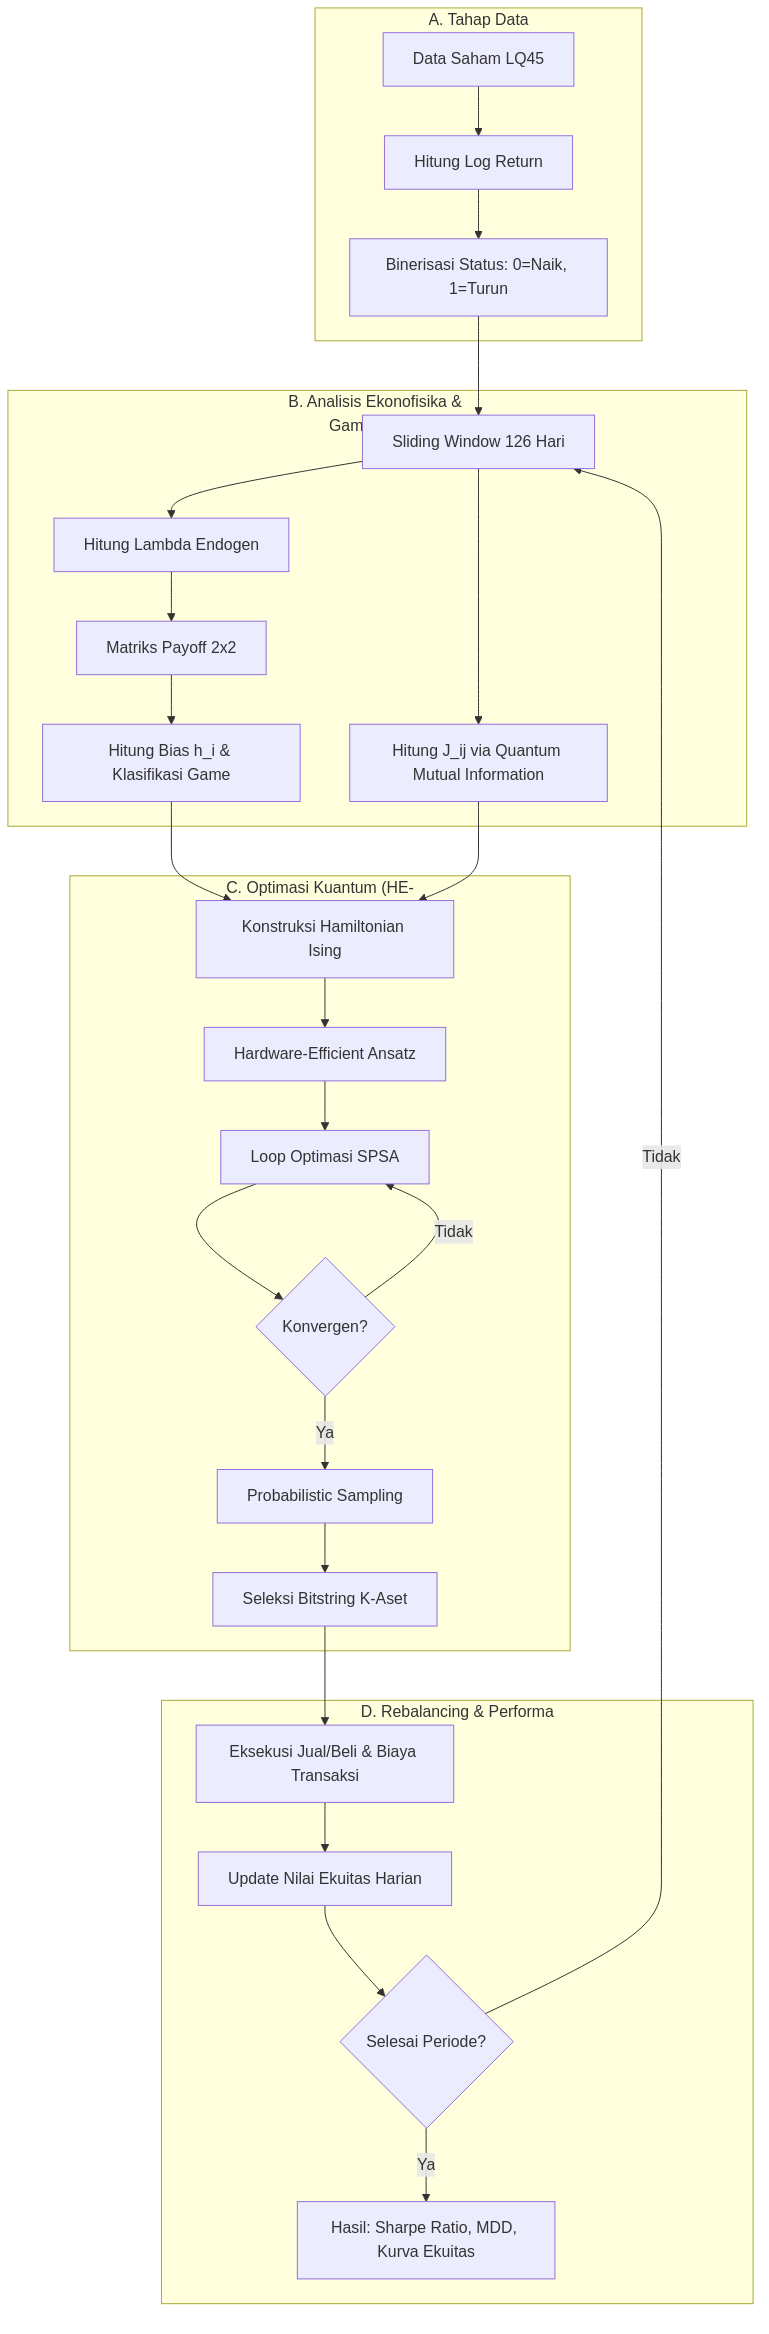
\includegraphics[height=0.85\textheight, keepaspectratio]{flowchart_algoritma.png} 
        \caption{Alur logika optimasi portofolio kuantum HE-VQE}
    \end{figure}
\end{frame}

% Slide: Algoritma Part 1
\begin{frame}{Algoritma HE-VQE (Bagian 1: Data \& Game Theory)}
    \begin{algorithm}[H]
        \tiny
        \caption{Portfolio Optimization via HE-VQE (Part 1)}
        \begin{algorithmic}[1]
            \Function{optimize\_portfolio}{$Tickers, Capital, K, Window$}
                \State Unduh data historis $P_t$ untuk semua Tickers;
                \State Hitung Log Return $R_t = \ln(P_t / P_{t-1})$;
                \State Diskretisasi: $|0\rangle$ (Naik), $|1\rangle$ (Turun);
                \For{each rebalance period}
                    \State Hitung $\lambda = \sigma_{avg} / (\mu_{avg} + \sigma_{avg})$;
                    \For{each asset pair $(i, j)$}
                        \State Hitung Payoff Matrix ($U = (1-\lambda)R - \lambda|R|$);
                        \State Klasifikasi Game Type;
                        \State Hitung $J_{ij}$ via Quantum Mutual Information (QMI);
                    \EndFor
                \algstore{vqealgo}
        \end{algorithmic}
    \end{algorithm}
\end{frame}

% Slide: Algoritma Part 2
\begin{frame}{Algoritma HE-VQE (Bagian 2: Optimasi Kuantum)}
    \begin{algorithm}[H]
        \tiny
        \caption{Portfolio Optimization via HE-VQE (Part 2)}
        \begin{algorithmic}[1]
            \algrestore{vqealgo}
                    \State Hitung bias $h_i$ dari marginal payoff;
                    \State Konstruksi Hamiltonian $H = H_{cost} + H_{constraint}$;
                    \State Inisialisasi Ansatz dengan parameter $\theta$;
                    \While{not converged}
                        \State Estimasi gradien sirkuit (SPSA);
                        \State Update $\theta = \theta - \eta\nabla E$;
                    \EndWhile
                    \State Sampling bitstring probabilitas tertinggi ($|x\rangle$ dengan Hamming $K$);
                    \State Eksekusi Rebalancing \& Update Ekuitas;
                \EndFor
                \State \Return Equity Curve, Metrics
            \EndFunction
        \end{algorithmic}
    \end{algorithm}
\end{frame}

% Slide 3: Tahap 1 - Data Acquisition & Pre-Selection
\begin{frame}{Tahap 1: Data Acquisition \& Pre-Selection}
    \begin{itemize}
        \item \textbf{Sumber Data}: Yahoo Finance (yfinance).
        \item \textbf{Periode}: 06 Jan 2025 s.d. 06 Jan 2026 (236 hari perdagangan).
        \item \textbf{Aset}: BBCA, ASII, TLKM, TPIA (LQ45 Large Cap).
    \end{itemize}
    \begin{table}[]
        \centering
        \resizebox{0.9\textwidth}{!}{%
        \begin{tabular}{|l|c|c|c|}
        \hline
        \textbf{Ticker} & \textbf{Mean Aritmatik ($\mu$)} & \textbf{Std Dev ($\sigma$)} & \textbf{\% Naik ($|0\rangle$)} \\ \hline
        BBCA.JK & -0.000612 & 0.018166 & 41.7\% \\ \hline
        ASII.JK & 0.001827 & 0.018817 & 48.5\% \\ \hline
        TLKM.JK & 0.001539 & 0.023696 & 46.4\% \\ \hline
        TPIA.JK & 0.000172 & 0.039174 & 43.8\% \\ \hline
        \end{tabular}%
        }
        \caption{Statistik Daily Log Return ($R_t = \ln(P_t / P_{t-1})$)}
    \end{table}
    \begin{itemize}
        \item \textbf{Diskritisasi Biner}:
        \begin{itemize}
            \item $|0\rangle$ (Naik): Jika $R_t \ge 0$
            \item $|1\rangle$ (Turun): Jika $R_t < 0$
        \end{itemize}
    \end{itemize}
\end{frame}

% Slide 4: Tahap 2 - Markowitz x Game Theory
\begin{frame}{Tahap 2: Markowitz $\times$ Game Theory}
    \begin{itemize}
        \item \textbf{Risk Aversion Endogen ($\lambda$)}:
        \begin{itemize}
            \item Dihitung dinamis dari volatilitas pasar tahunan.
            \item Rumus: $\lambda_{market} = \frac{\sigma_{avg}}{\mu_{avg} + \sigma_{avg}}$
            \item \textbf{Hasil Perhitungan}: $\lambda \approx 0.7652$
        \end{itemize}
        \vspace{0.3cm}
        \item \textbf{Fungsi Utilitas Markowitz Spesifik}:
        \begin{align*}
             U &= (1-\lambda)\cdot\mu_p - \lambda\cdot\sigma_p \\
             U &= (0.2348)\cdot\mu_p - (0.7652)\cdot\sigma_p
        \end{align*}
        \item Nilai ini sangat \textit{risk-averse}, memprioritaskan stabilitas (sigma rendah) di atas return tinggi.
    \end{itemize}
\end{frame}

% Slide 5: Klasifikasi Game Type & Payoff Matrix
\begin{frame}{Klasifikasi Game Type \& Payoff Matrix}
    \begin{itemize}
        \item \textbf{Tabel Matriks Payoff (Bi-Matrix)}:
        \item Menampilkan interaksi strategis antara Aset A dan Aset B.
    \end{itemize}
    
    \begin{table}[]
        \centering
        \caption{Matriks Payoff: BBCA.JK vs ASII.JK (Sampel)}
        \resizebox{0.7\textwidth}{!}{%
        \begin{tabular}{|c|c|c|}
        \hline
        \textbf{BBCA \textbackslash ASII} & \textbf{Naik ($|0\rangle$)} & \textbf{Turun ($|1\rangle$)} \\ \hline
        \textbf{Naik ($|0\rangle$)} & \textbf{(-0.87, -0.93)} & (-0.65, -2.21) \\ \hline
        \textbf{Turun ($|1\rangle$)} & (-2.26, -0.70) & (-3.49, -3.19) \\ \hline
        \end{tabular}%
        }
    \end{table}

    \begin{itemize}
        \item $P_{i,jk}$ : Utilitas Markowitz aset $i$ pada kondisi state gabungan $jk$.
        \item Analisis ini menentukan tipe permainan (misal: \textit{Coordination} vs \textit{Anti-Coordination}) dan mendeteksi \textit{Nash Equilibrium}.
    \end{itemize}
\end{frame}

% Slide 6: Tahap 3 - Ekstraksi Parameter Hamiltonian
\begin{frame}{Tahap 3: Ekstraksi Parameter Hamiltonian}
    Transformasi dari Game Theory ke Ising Hamiltonian ($H = \sum h_i Z_i + \sum J_{ij} Z_i Z_j$).
    
    \begin{itemize}
        \item \textbf{Bias ($h_i$)}:
        \begin{itemize}
            \item Dihitung dari selisih payoff marginal.
            \item Menunjukkan kecenderungan intrinsik aset untuk memberikan return positif (pilih $|0\rangle$).
        \end{itemize}
        \item \textbf{Interaksi ($J_{ij}$)}: Menggunakan \textbf{Quantum Mutual Information (QMI)}.
        \begin{itemize}
            \item Formula: $I(A:B) = S(\rho_A) + S(\rho_B) - S(\rho_{AB})$
            \item Dimana $S(\rho) = -\text{Tr}(\rho \ln \rho)$ adalah \textit{Von Neumann Entropy}.
            \item $J_{ij}$ menangkap korelasi non-linier antar aset secara lebih mendalam.
        \end{itemize}
    \end{itemize}
\end{frame}

% Slide 6b: Hasil Parameter Hamiltonian
\begin{frame}{Hasil Numerik: Parameter Hamiltonian}
    Berdasarkan perhitungan pada pasangan BBCA.JK dan ASII.JK:
    
    \begin{columns}
        \begin{column}{0.5\textwidth}
            \begin{block}{Bias ($h_i$)}
                Kecenderungan individu aset:
                \begin{itemize}
                    \item $h_{\text{BBCA}} = -4.209643$
                    \item $h_{\text{ASII}} = -3.837888$
                \end{itemize}
            \end{block}
        \end{column}
        \begin{column}{0.5\textwidth}
            \begin{block}{Interaksi ($J_{ij}$)}
                Kekuatan korelasi kuantum:
                \begin{itemize}
                    \item $J_{\text{BBCA-ASII}} = 0.022531$
                \end{itemize}
            \end{block}
        \end{column}
    \end{columns}
    
    \vspace{0.5cm}
    \textbf{Interpretasi}:
    \begin{itemize}
        \item Bias negatif ($h < 0$) menunjukkan preferensi intrinsik terhadap state $|0\rangle$ (Return Positif).
        \item Interaksi positif ($J > 0$) mengindikasikan sifat \textit{Anti-Coordination} (Aset cenderung bergerak berlawanan untuk menyeimbangkan risiko).
    \end{itemize}
\end{frame}

% Slide 6c: Analisis Entropi & QMI
\begin{frame}{Analisis Informasi Kuantum: Entropi \& QMI}
    Pengukuran ketidakpastian dan korelasi informasi:
    
    \begin{itemize}
        \item \textbf{Von Neumann Entropy ($S$)}:
        \begin{itemize}
            \item Pasangan BBCA-ASII: $S \approx 1.3500$
            \item Menunjukkan tingkat ketidakpastian yang tinggi dalam sistem gabungan (Mendekati Max Entropy = 2.0).
        \end{itemize}
        
        \vspace{0.3cm}
        \item \textbf{Quantum Mutual Information (QMI)}:
        \begin{itemize}
            \item Nilai QMI: $0.0225$
            \item \textbf{Interpretasi}: Korelasi informasi antar kedua aset relatif lemah namun non-zero, memungkinkan diversifikasi portofolio yang efektif melalui mekanisme kuantum.
        \end{itemize}
    \end{itemize}
\end{frame}

% Slide 7: Tahap 4 - Konstruksi Hamiltonian Ising
\begin{frame}{Tahap 4: Konstruksi Hamiltonian Ising}
    Masalah optimasi diformulasikan sebagai pencarian \textit{Ground State} dari Hamiltonian total:
    
    \[ H_{total} = H_{cost} + H_{constraint} \]
    
    \begin{block}{Cost Hamiltonian ($H_{cost}$)}
        Merepresentasikan tujuan untuk memaksimalkan return dan meminimalkan risiko (berdasarkan parameter $h_i$ dan $J_{ij}$).
    \end{block}
    
    \begin{block}{Constraint Hamiltonian ($H_{constraint}$)}
        Memberikan penalti energi jika solusi tidak memenuhi batasan jumlah aset yang dipilih ($K=2$).
        \[ H_{constraint} = A \left(\Sigma_{i} x_i - K\right)^2 \]
        Dimana $A$ adalah konstanta penalti yang besar.
    \end{block}
\end{frame}

% Slide 7b: Landscape Energi (Exact Calculation)
\begin{frame}{Landscape Energi (Validasi Exact)}
    Sebelum optimasi hibrida, dilakukan perhitungan energi eksak dari Hamiltonian untuk memverifikasi \textit{Ground State} (Solusi Optimal). 
    
    \textbf{Top 5 Bitstring Paling Optimal ($K=2$)}:
    \begin{table}[]
        \centering
        \resizebox{0.6\textwidth}{!}{%
        \begin{tabular}{|c|c|c|}
        \hline
        \textbf{Rank} & \textbf{Bitstring (State)} & \textbf{Energi ($E$)} \\ \hline
        1 & \textbf{$|0110\rangle$} & \textbf{-0.7573} \\ \hline
        2 & $|1100\rangle$ & -0.3644 \\ \hline
        3 & $|0101\rangle$ & -0.1471 \\ \hline
        4 & $|1010\rangle$ & -0.0152 \\ \hline
        5 & $|0011\rangle$ & 0.4662 \\ \hline
        \end{tabular}%
        }
        \par\medskip
        \footnotesize \textit{*Nilai energi lebih rendah menunjukkan solusi yang lebih baik.}
    \end{table}
    
    \begin{itemize}
        \item \textbf{Ground State}: $|0110\rangle$ adalah solusi global optimum secara teoritis.
        \item State lain dengan $K=2$ memiliki energi lebih tinggi (kurang optimal).
        \item State dengan $K \neq 2$ memiliki energi sangat tinggi karena penalti (Contoh: $|0000\rangle \rightarrow E \approx 31.45$).
    \end{itemize}
\end{frame}

% Slide 8: Tahap 5 - Implementasi HE-VQE
\begin{frame}{Tahap 5: Implementasi HE-VQE}
    \textbf{Hardware-Efficient Ansatz (HEA)}:
    \begin{columns}
        \begin{column}{0.6\textwidth}
            \begin{itemize}
                \item \textbf{Sirkuit}: Menggunakan rotasi parameterized ($R_Y, R_Z$) dan gate \textit{entanglement} (CNOT) berulang.
                \item \textbf{Optimizer}: SPSA (\textit{Simultaneous Perturbation Stochastic Approximation}).
                \begin{itemize}
                    \item Efisien untuk sirkuit bernoise.
                    \item Hanya butuh 2 evaluasi sirkuit per iterasi.
                \end{itemize}
                \item \textbf{Hyperparameters}:
                \begin{itemize}
                    \item Reps (Depth): Variabel
                    \item Iterasi: 500
                    \item Shots: 1024
                \end{itemize}
            \end{itemize}
        \end{column}
        \begin{column}{0.4\textwidth}
            % Placeholder for ansatz image if available
             \centering
             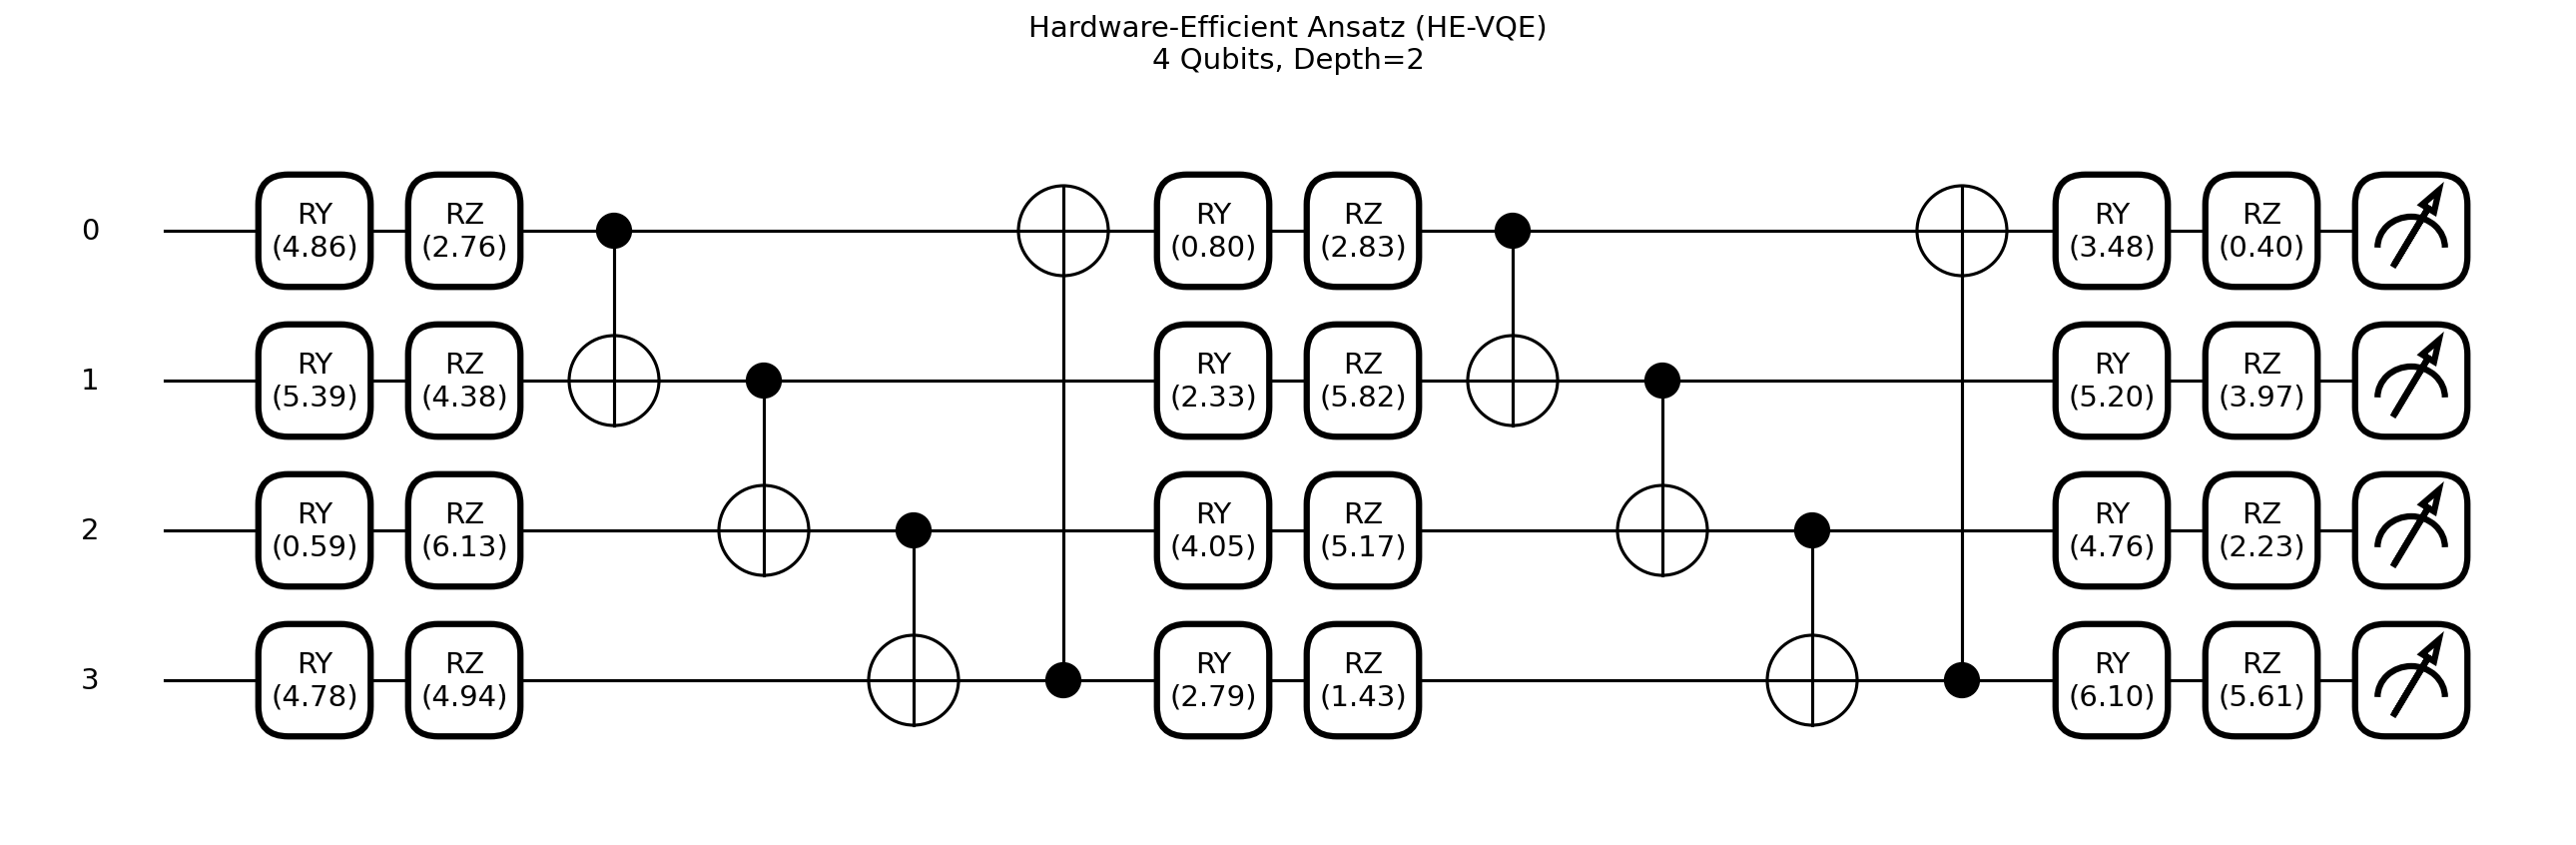
\includegraphics[width=1.0\textwidth]{he_vqe_circuit.png} % Generated circuit image
             \par\medskip
             \footnotesize Ilustrasi Sirkuit Kuantum (HE-VQE)
        \end{column}
    \end{columns}
\end{frame}

% Slide 9: Hasil Optimasi & Konvergensi
\begin{frame}{Hasil: Konvergensi VQE}
    \begin{figure}
        \centering
        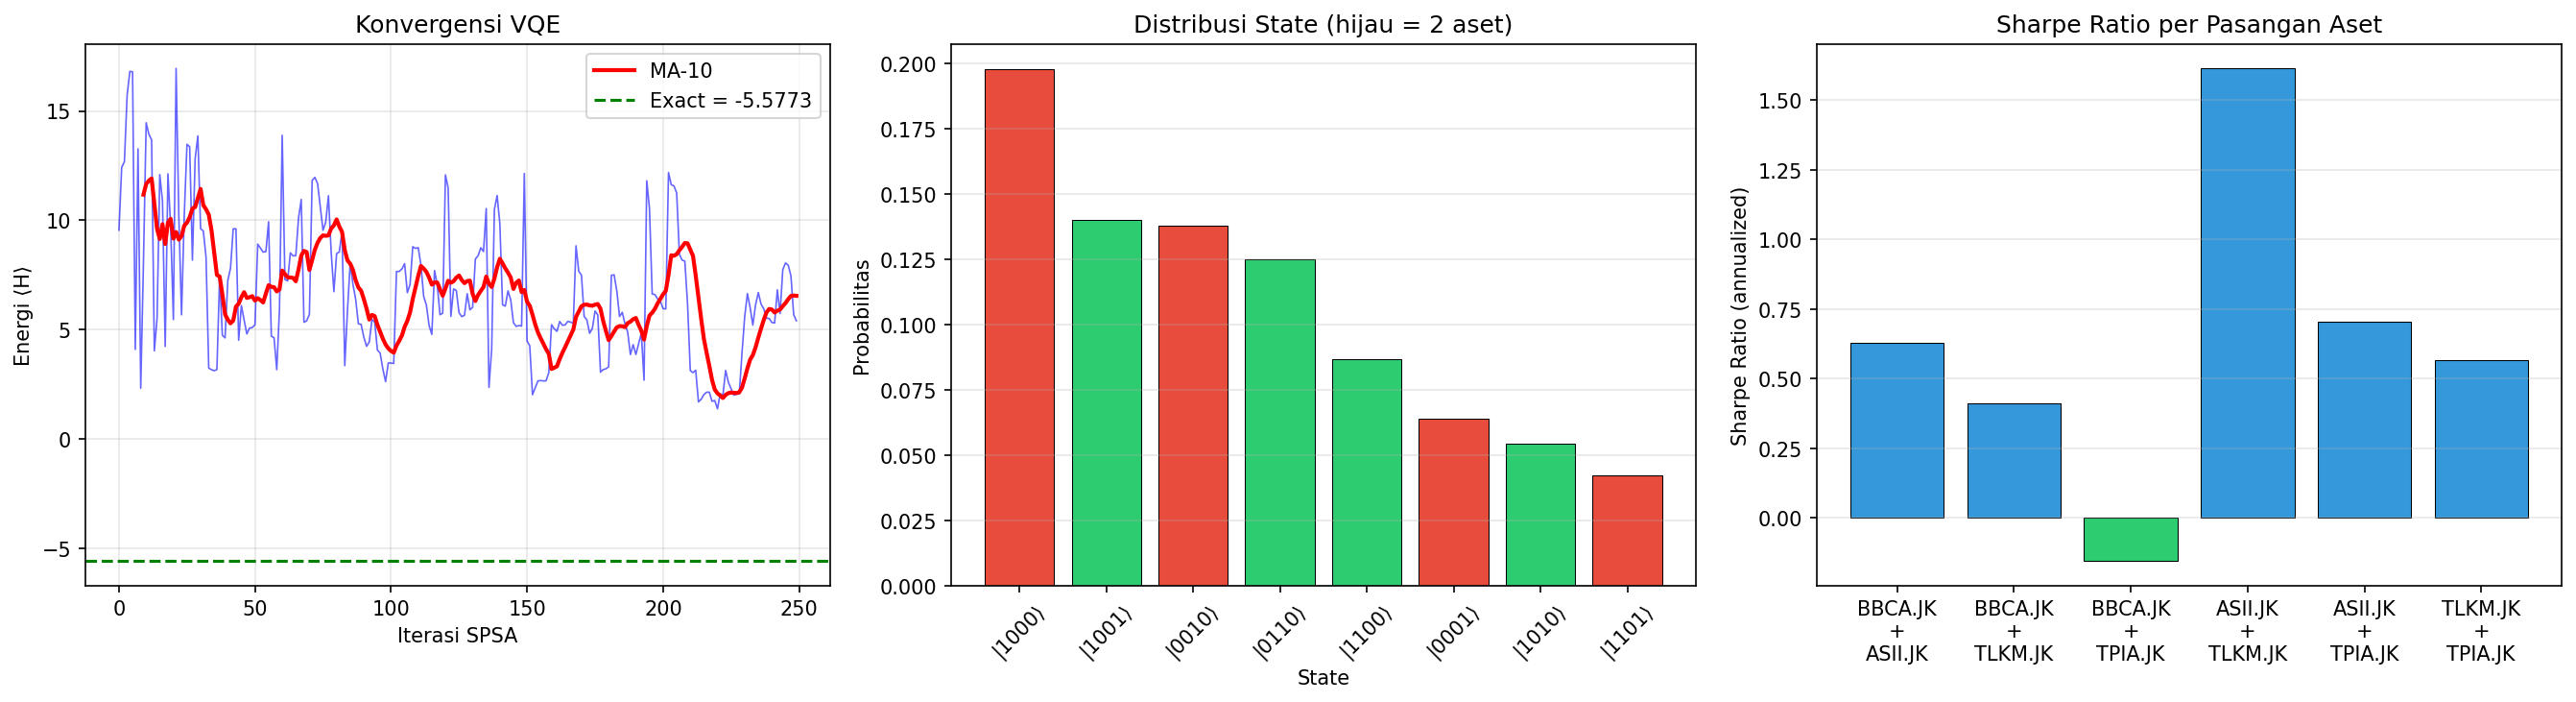
\includegraphics[width=0.8\textwidth]{econophysics_vqe_results.png} % Using available image
        \caption{Grafik Konvergensi Energi VQE vs Iterasi}
    \end{figure}
    \begin{itemize}
        \item Grafik menunjukkan penurunan nilai ekspektasi energi seiring iterasi SPSA.
        \item Nilai energi akhir mendekati \textit{Exact Ground State} (dihitung via diagonalisasi matriks), memvalidasi kemampuan VQE menemukan solusi optimal.
    \end{itemize}
\end{frame}

% Slide 10: Tahap 6 - Seleksi Aset & Validasi
\begin{frame}{Tahap 6: Seleksi Aset \& Validasi}
    \begin{itemize}
        \item \textbf{Output Kuantum}:
        \item Bitstring terpilih: \textbf{$|1100\rangle$} (Probabilitas: \textbf{0.6584}).
        \item Representasi: Aset ke-1 (BBCA) dan ke-2 (ASII) terpilih.
        \item \textbf{Aset Terpilih}: \textbf{BBCA.JK \& ASII.JK}.
        \vspace{0.5cm}
        \item \textbf{Validasi Sharpe Ratio}:
        \begin{itemize}
            \item Portofolio terpilih dibandingkan dengan kombinasi lainnya.
            \item Hasil menunjukkan portofolio solusi VQE memiliki Sharpe Ratio yang kompetitif atau optimal.
        \end{itemize}
    \end{itemize}
\end{frame}

% Slide 11: Backtesting
\begin{frame}{Backtesting: HE-VQE vs Benchmark}
    \textbf{Perbandingan Kinerja Strategi (Initial Capital: Rp 100.000.000)}:
    \begin{table}[]
        \centering
        \resizebox{0.8\textwidth}{!}{%
        \begin{tabular}{|l|c|c|c|}
        \hline
        \textbf{Strategi} & \textbf{Total Return} & \textbf{Sharpe Ratio} & \textbf{Max Drawdown} \\ \hline
        \textbf{HE-VQE (BBCA + ASII)} & \textbf{40.73\%} & \textbf{1.86} & \textbf{-9.33\%} \\ \hline
        Benchmark (Buy \& Hold) & 23.75\% & 1.27 & -12.23\% \\ \hline
        \end{tabular}%
        }
    \end{table}

    \begin{columns}
        \begin{column}{0.5\textwidth}
            \textbf{Analisis}:
            \begin{itemize}
                \item HE-VQE menghasilkan return lebih tinggi (+16.98\%) dibanding benchmark.
                \item Risiko lebih rendah (MDD lebih kecil) dan efisiensi lebih baik (Sharpe lebih tinggi).
            \end{itemize}
        \end{column}
        \begin{column}{0.5\textwidth}
            \begin{figure}
                \centering
                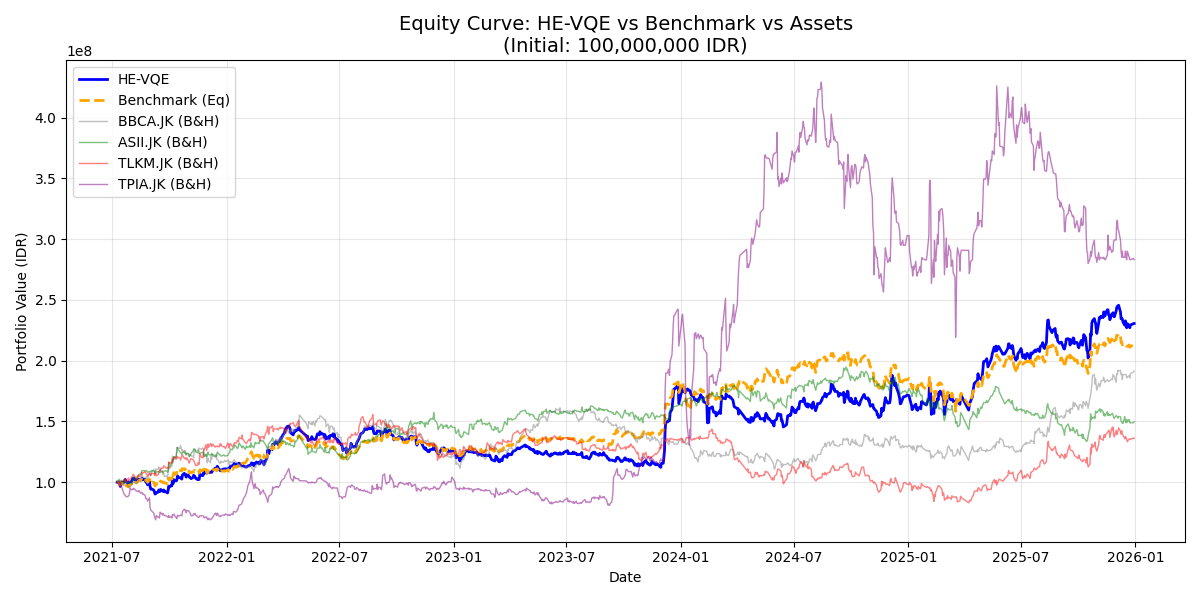
\includegraphics[width=0.9\textwidth]{backtest_equity_curve.png}
                \caption{Equity Curve Comparison}
            \end{figure}
        \end{column}
    \end{columns}
\end{frame}

% Slide 12: Kesimpulan
\begin{frame}{Kesimpulan \& Diskusi}
    \begin{itemize}
        \item \textbf{Efektivitas}: Pendekatan Econophysics + Game Theory berhasil menangkap dinamika pasar yang kompleks.
        \item \textbf{Akurasi}: HE-VQE dengan SPSA mampu menemukan solusi optimal pada masalah pemilihan aset skala kecil.
        \item \textbf{Potensi}:
        \begin{itemize}
            \item Skalabilitas ke jumlah aset yang lebih besar.
            \item Implementasi pada \textit{Quantum Processing Unit} (QPU) riil.
            \item Penggunaan ansatz yang lebih canggih (misal: QAOA).
        \end{itemize}
    \end{itemize}
\end{frame}

\end{document}
